\section{Repérage (4 points)}

Dans la grille ci-dessous :

\begin{multicols}{2}
	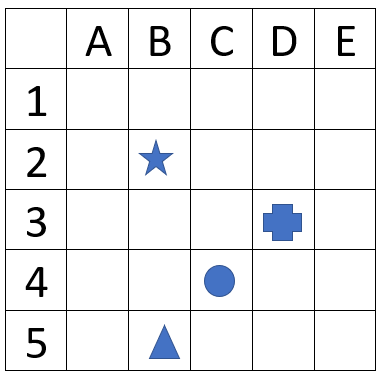
\includegraphics[scale=0.5]{img/grille}
	
	\begin{questions}
		\question[1] Donner les coordonnées de chaque symbole.
		
		\question[1\half] Placer en bleu \textbf{dans cette grille} la nouvelle position du triangle après les mouvements suivants :  {\Large $\Rightarrow \; \Rightarrow \; \Uparrow  \; \Uparrow \; \Leftarrow$}.
		
		\question[1\half] Quels mouvement devrait-il faire \textbf{depuis sa nouvelle position} pour arriver en $A2$.
	\end{questions}
\end{multicols}

